% mhchem.tex
%
% Copyright (C) 2022--2026 José A. Navarro Ramón <janr.devel@gmail.com>
% Licencia del código GPLv2
% Licencia Creative Commons Recognition Non-Commercial Share-alike.
% (CC-BY-NC-SA)


\chapter{Paquete {\sf{mhchem}}}
Este capítulo tiene los siguientes objetivos:
\begin{enumerate}
\item Aprender cómo cargar el paquete en Lua\LaTeX.
\item Familiarizarse con sus principales características, sobre todo las que se aplican
  en un contexto de ESO y bachillerato.
\item Conocer algunas formas de modificar algunas características que presenta por
  defecto el paquete.
\item Conocer sus puntos fuertes y carencias.
\end{enumerate}

\section{Introducción}
En esta sección veremos algunos detalles importantes para usar este paquete.

\subsection{¿Cuándo interesa utilizarlo?}
Es el paquete más sencillo que repasaremos.
Sirve para escribir:
\begin{enumerate}
\item Fórmulas químicas (orgánica e inorgánica) en una línea.
\item Reacciones químicas que se escriben en una línea.
\end{enumerate}

\subsection{Carga del paquete}
Para poder utilizarlo es preciso cargarlo en el preámbulo del documento, esto es,
antes de \texttt{\textbackslash begin\{document\}...\textbackslash end\{document\}}.

Se pueden dar dos situaciones:
\vspace{-1ex}
\begin{itemize}
\item Si \textsf{mhchem} se carga en el fichero principal:
  \textcolor{red!70!black}{\texttt{\textbackslash usepackage[version=4]\{mhchem\}}}
\item Si queremos que el fichero principal se vea más ordenado, entonces se debe
  indicar qué otro fichero realizará la carga, en cuyo caso se deberá escribir en
  el principal la línea: 
  \textcolor{red!70!black}{\texttt{\textbackslash usepackage\{fichero.pkg\}}} en el
  principal, indicando que el fichero que realizará la carga será 
 \texttt{fichero.pkg.sty}. En este último hay que añadir una línea que ponga:
 \textcolor{red!70!black}{\texttt{\textbackslash RequirePackage[version=4]\{mhchem\}}},
 además del resto de paquetes que nos interese cargar.
\end{itemize}

%\begin{figure}[ht]
%  \pgfmathsetmacro{\EJESNEGLONG}{0.2}
%  \pgfmathsetmacro{\EJESPOSLONG}{2.3}
%  % Eje x
%  \pgfmathsetmacro{\XNEGLONG}{\EJESNEGLONG}
%  \pgfmathsetmacro{\XPOSLONG}{\EJESPOSLONG}
%  % Eje y
%  \pgfmathsetmacro{\YNEGLONG}{\EJESNEGLONG}
%  \pgfmathsetmacro{\YPOSLONG}{\EJESPOSLONG}
%  % Versores
%  \pgfmathsetmacro{\VERSORMOD}{0.6}
%  % Vector P
%  \pgfmathsetmacro{\VECTORMOD}{2.5}
%  \pgfmathsetmacro{\VECTORANG}{40}
%  % Fondo
%  \pgfmathsetmacro{\HORZ}{0.25}
%  \pgfmathsetmacro{\VERT}{0.25}
%  % 
%  \centering
%  \begin{tikzpicture}[%
%    scale=1,
%    every node/.style={black,font=\footnotesize},
%    eje/.style={->},
%    proyeccion/.style={black!20, line width=0.4},
%    vector/.style={-{Latex[round]}, shorten >=1.2pt, line width=.8pt, black},
%    versor/.style={-{Latex[round, width=4pt, length=6pt]}, line width=1pt, red!80!black},
%    texto/.style={black},
%    pcirculo/.style={fill=green, draw=black},
%    background/.style={%
%      line width=\backgrounborderwidth,
%      draw=\backgroundbordercolor,
%      fill=\backgroundcolor,
%    },
%    ]
%    % -------------------------------------------------------------------------------
%    % COORDENADAS
%    % Origen
%    \coordinate (O) at (0,0);
%    % Extremo izdo del eje x e inferior del eje y
%    \coordinate (xini) at (-\XNEGLONG,0);
%    \coordinate (yini) at (0,-\YNEGLONG);
%    \coordinate (ifin) at (\VERSORMOD, 0);
%    \coordinate (jfin) at (0, \VERSORMOD);
%    % Eje x
%    \path[save path=\ejex] (xini) -- coordinate[pos=0.55] (xtexto) (\XPOSLONG, 0)
%    coordinate (xfin);
%    % Eje y
%    \path[save path=\ejey] (yini) -- coordinate[pos=0.55] (ytexto) (0, \YPOSLONG)
%    coordinate (yfin);
%    % Versores i y j
%    \path[save path=\ivector] (O) -- coordinate[pos=0.5] (itexto) (ifin);
%    \path[save path=\jvector] (O) -- coordinate[pos=0.45] (jtexto) (jfin);    
%    % Vector
%    \path[save path=\vector] (O) -- coordinate[pos=0.5] (pmid) (\VECTORANG:\VECTORMOD)
%    coordinate (P);
%    % Proyección de P en los ejes
%    \path[save path=\proyx] (P) |- (xfin);
%    \path[save path=\proyy] (P) -| (yfin);
%% -------------------------------------------------------------------------------
%    % DIBUJOS
%    % Proyección de P en los ejes
%    \draw[proyeccion, use path=\proyx];
%    \draw[proyeccion, use path=\proyy];
%    % Ejes
%    % x
%    \draw[eje, use path=\ejex];
%    \node[right] at (xfin) {$x$};
%    \node[below] at (xtexto) {$x$};
%    % y
%    \draw[eje, use path=\ejey];
%    \node[above] at (yfin) {$y$};
%    \node[left] at (ytexto) {$y$};
%    % Versores
%    \draw[versor, use path=\ivector];
%    \node[below, red!80!black] at (itexto) {hola};
%    \draw[versor, use path=\jvector];
%    \node[left, red!80!black] at (jtexto) {hola};
%    % Vector y punto  P
%    \draw[vector, use path=\vector];
%    \node[above left=-3pt and -1pt] at (pmid) {$r$};
%    \filldraw[fill=green, draw=black] (P) circle[radius=1.2pt];
%    \node[above right=0pt and -5pt] at (P) {$P(x,y)$};
%    
%    % Origen
%    \filldraw (O) circle [radius=.25pt];
%%    % -------------------------------------------------------------------------------    
%%    % Fondo amarillo
%%    \coordinate (SW) at ($(current bounding box.south west) + (-\HORZ cm,-\VERT cm)$);
%%    \coordinate (NE) at ($(current bounding box.north east) + (\HORZ cm,\VERT cm)$);    
%%    \begin{scope}[on background layer]
%%      \draw[background] (SW) rectangle (NE);
%%    \end{scope}
%  \end{tikzpicture}
%  \caption{Coordenadas cartesianas rectangulares de un punto $P$ del plano
%    (en verde) y vectores unitarios (en rojo). El vector de posición del punto
%    es $r$.}
%  %\label{fig:R2-rect_ij}
%\end{figure}


%% Define box and box title style
%\tikzstyle{mybox} = [draw=red, fill=blue!20, very thick,
%    rectangle, rounded corners, inner sep=10pt, inner ysep=20pt]
%\tikzstyle{fancytitle} =[fill=red, text=white]


\vspace{3ex}

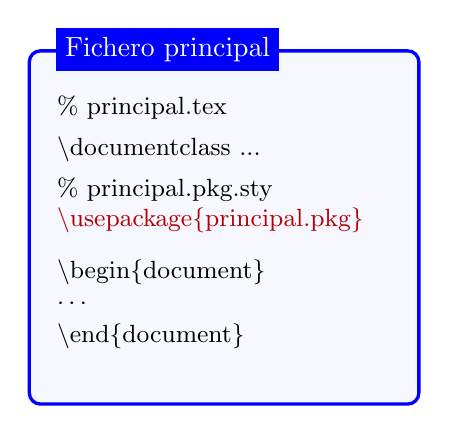
\begin{tikzpicture}
  % Define box and box title style
  \tikzstyle{myboxfichero} = [draw=blue, fill=blue!3, very thick,
  rectangle, rounded corners, inner sep=10pt, inner ysep=20pt]
  \tikzstyle{fancytitle} =[fill=blue, text=white]
    
  \node [myboxfichero] (box){%
    \begin{minipage}{0.35\textwidth}
      {\small
        
        \vspace{-1ex}
        \% principal.tex
        
        \vspace{1ex}
        
        \textbackslash documentclass ...
        
        \vspace{1ex}
        
        \% principal.pkg.sty
        
        \textcolor{red!70!black}{\textbackslash usepackage\{principal.pkg\}}
        
        \vspace{2ex}
        
        \textbackslash begin\{document\}
        
        $\cdots$
        
        \textbackslash end\{document\}
      }
    \end{minipage}
  };

  \node[fancytitle, right=10pt] at (box.north west) {Fichero principal};
  % \node[fancytitle, rounded corners] at (box.east) {$\clubsuit$};
\end{tikzpicture}%
%
\hspace{1em}
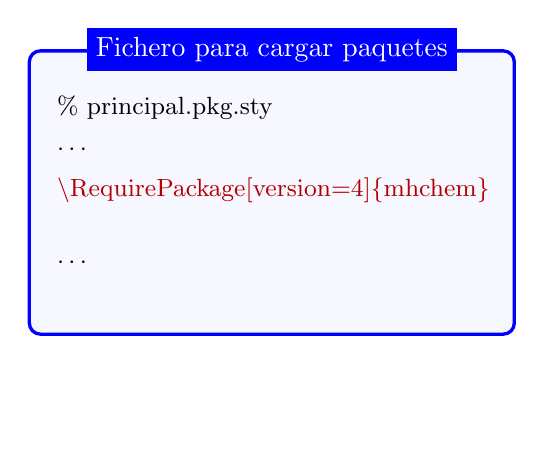
\begin{tikzpicture}[transform shape, rotate=0, baseline=-2.9cm]
  % Define box and box title style
  \tikzstyle{myboxfichero} = [draw=blue, fill=blue!3, very thick,
  rectangle, rounded corners, inner sep=10pt, inner ysep=20pt]
  \tikzstyle{fancytitle} =[fill=blue, text=white]
  
  \node [myboxfichero] (box) {%
    \begin{minipage}[t!]{0.45\textwidth}
      {\small
        \vspace{-1ex}
        \% principal.pkg.sty
        
        \vspace{1ex}
        
        $\cdots$
        \vspace{1ex}
        
        \textcolor{red!70!black}{\textbackslash RequirePackage[version=4]\{mhchem\}}
        \vspace{1ex}
        
        $\cdots$
        
        \vspace{1ex}
      }
    \end{minipage}
  };
  \node[fancytitle] at (box.north) {Fichero para cargar paquetes};
\end{tikzpicture}
%

\subsection{Uso del paquete}
El comando básico es \texttt{\textbackslash ce\{...\}}.
En las siguientes secciones veremos ejemplos de uso.

\section{Átomos, sustancias y derivados}
En esta sección empezaremos a escribir las fórmulas de átomos, isótopos, elementos,
compuestos y derivados.

\subsection{Átomos neutros}
Se escribe el símbolo del átomo como argumento del comando
\texttt{\textbackslash ce\{...\}}. Si queremos especificar el estado físico, podemos
escribirlo entre paréntesis, tal y como recomienda la IUPAC, y no como subíndice.


\vspace{1ex}
\begin{tabular}{|c|c|c|c|c|}\hline
  \phantom{$\int{}$}
\ce{H} & \ce{As} & \ce{Na(s)} & \ce{X(g)} & \ce{C(s)}\\
  \texttt{\textbackslash ce\{H\}}
       & \texttt{\textbackslash ce\{As\}}
       & \texttt{\textbackslash ce\{Na(s)\}}
       & \texttt{\textbackslash ce\{Xe(g)\}}
       & \texttt{\textbackslash ce\{C(s)\}\$}\\\hline
\end{tabular}


\subsection{Sustancias neutras}
Además, de algunas que se han mostrado arriba, podemos escribir moléculas, compuestos
iónicos, etc. Los subíndices numéricos se indican mediante el número sin necesidad del
subrayado, aunque también se puede utilizar con él. Si el subíndice no es totalmente
numérico es obligatorio el subrayado:

\vspace{1ex}
\begin{tabular}{|c|c|c|c|c|}\hline
  \phantom{$\dfrac{1}{1}$}
\ce{KCl} & \ce{PbS2} & \ce{Cu2SO3} & \ce{C7H14} & \ce{C_nH_{2n+2}}\\
  \texttt{\textbackslash ce\{KCl\}}
       & \texttt{\textbackslash ce\{PbS2\}}
       & \texttt{\textbackslash ce\{Cu2SO3\}}
       & \texttt{\textbackslash ce\{C7H14\}}                        
       & \texttt{\textbackslash ce\{C\_nH\_\{2n+2\}\}}\\\hline
\end{tabular}

\vspace{2ex}
\begin{tabular}{|c|c|c|c|}\hline
  \phantom{$\dfrac{1}{1}$}
\ce{CH4(g)} & \ce{NaCl(s)} & \ce{H2O(l)} & \ce{N2(g)} \\
  \texttt{\textbackslash ce\{CH4(g)\}}
       & \texttt{\textbackslash ce\{NaCl(s)\}}
       & \texttt{\textbackslash ce\{H2O(l)\}}
       & \texttt{\textbackslash ce\{N2(g)\}}\\\hline
\end{tabular}

%\pagebreak
\vspace{1ex}
Las sales hidratadas se escriben con el asterisco \texttt{(*)} o el punto \texttt{.}:

\vspace{1ex}
\begin{tabular}{|c|c|c|}\hline
  \phantom{$\dfrac{1}{1}$}
\ce{CuSO4*5H2O} & \ce{CaSO4.2H2O(s)} & \ce{CoCl2*6H2O}\\
  \texttt{\textbackslash ce\{CuSO4*5H2O\}}
       & \texttt{\textbackslash ce\{CaSO4.2H2O(s)\}}
       & \texttt{\textbackslash ce\{CoCl2*6H2O\}}\\\hline
\end{tabular}

\subsection{Enlaces químicos}
\subsubsection{Sencillos, dobles y triples}
Los enlaces sencillos se indican mediante el guión o signo negativo \texttt{-},
los dobles mediante el carácter \texttt{=} y el triple mediante \texttt{\#}:

\vspace{1ex}
\begin{tabular}{|c|c|c|c|}\hline
\phantom{$\dfrac{1}{1}$}  
\ce{CH2=CH-CH3(g)} & \ce{CH#CH(g)} & \ce{CH3NH2} & \ce{C6H5-CH3} \\
  \texttt{\textbackslash ce\{CH2=CH-CH3(g)\}}
       & \texttt{\textbackslash ce\{CH\#CH\{g\}\}}
       & \texttt{\textbackslash ce\{CH3NH2\}}
       & \texttt{\textbackslash ce\{C6H5-CH3\}}\\\hline
\end{tabular}

\vspace{2ex}
En algunas ocasiones {\sffamily mhchem} podría confundir alguno de los caracteres anteriores
y no producir los enlaces deseados, debido a que debe interpretar si \texttt{-}, por
ejemplo, es un guión, el signo negativo o un enlace sencillo. Para solucionar
malinterpretaciones, se podría utilizar en su lugar
\texttt{\textbackslash bond\{-\}},
\texttt{\textbackslash bond\{=\}}
y \texttt{\textbackslash bond\{\#\}}:

\vspace{1ex}
\begin{tabular}{|c|c|c|}\hline
\phantom{$\dfrac{1}{1}$}  
\ce{CH2\bond{=}CH2} & \ce{CH\bond{#}CH} & \ce{CH3\bond{-}CH3} \\
  \texttt{\textbackslash ce\{CH2\textbackslash bond\{=\}CH2\}}
       & \texttt{\textbackslash ce\{CH\textbackslash bond\{\#\}CH\}}
       & \texttt{\textbackslash ce\{CH3\textbackslash bond\{-\}CH3\}}\\\hline
\end{tabular}

\vspace{2ex}
Si no se corrigiera así, se podría poner
\texttt{\textbackslash bond\{1\}},
\texttt{\textbackslash bond\{2\}} y
\texttt{\textbackslash bond\{3\}}:

\vspace{1ex}
\begin{tabular}{|c|c|c|}\hline
\phantom{$\dfrac{1}{1}$}  
\ce{CH2\bond{2}CH2} & \ce{CH\bond{3}CH} & \ce{CH3\bond{1}CH3} \\
  \texttt{\textbackslash ce\{CH2\textbackslash bond\{2\}CH2\}}
       & \texttt{\textbackslash ce\{CH\textbackslash bond\{3\}CH\}}
       & \texttt{\textbackslash ce\{CH3\textbackslash bond\{1\}CH3\}}\\\hline
\end{tabular}

\vspace{2ex}
Además, según se interprete \texttt{-} y sobre todo el tipo de letra que se utilice,
podría tener diferentes tamaños, lo que podría suponer un problema. Para resolver esto se
podría definir su longitud mediante:

{\footnotesize
  
\texttt{\textbackslash mhchemoptions\{minus-text-sidebearing-left=0.10em, minus-text-sidebearing-right=0.16em\}}
}
 para el uso de \texttt{\textbackslash ce\{...\}} en modo texto y

{\footnotesize
  
\texttt{\textbackslash mhchemoptions\{minus-math-sidebearing-left=0.06em, minus-math-sidebearing-right=0.11em\}}
}
 en modo matemático.


\subsubsection{Enlace covalente coordinado}
Este enlace se indica mediante \texttt{\textbackslash bond\{->\}} o
\texttt{\textbackslash bond\{<-\}}, según interese:

\vspace{1ex}
\begin{tabular}{|c|c|c|}\hline
\phantom{$\dfrac{1}{1}$}  
\ce{NH3\bond{<-}H+} & \ce{H+\bond{->}H2O} & \ce{BF3\bond{<-}F-} \\
  \texttt{\textbackslash ce\{CH2\textbackslash bond\{2\}CH2\}}
       & \texttt{\textbackslash ce\{CH\textbackslash bond\{3\}CH\}}
       & \texttt{\textbackslash ce\{CH3\textbackslash bond\{1\}CH3\}}\\\hline
\end{tabular}

\subsubsection{Enlace por puente de hidrógeno}
Este enlace se indica mediante tres puntos \texttt{\textbackslash bond\{...\}}:

\vspace{1ex}
\begin{tabular}{|c|c|}\hline
\phantom{$\dfrac{1}{1}$}  
\ce{A\bond{...}B} & \ce{HF\bond{...}HF\bond{...}HF} \\
  \texttt{\textbackslash ce\{A\textbackslash bond\{...\}B\}}
  & \texttt{%
      \textbackslash ce\{HF\textbackslash bond\{...\}HF\textbackslash\{...\}HF\}
    }\\\hline
\end{tabular}

\subsubsection{Enlace a medio crear/destruir}
Se indica mediante tres guiones cortos seguidos
\texttt{\textbackslash bond\{\textasciitilde\}}, aunque {\sffamily mhchem} solo permite
una línea y el ejemplo que sigue no es del todo preciso, pues debería representarse en
dos dimensiones, por lo que se recomienda otro paquete de química más completo:

\vspace{1ex}
\begin{tabular}{|c|}\hline
\phantom{$\dfrac{1}{1}$}  
\ce{2 H-I -> 2H\bond{~}I -> H2 + I2} \\
  \texttt{%
   \textbackslash ce\{2 H-I\textbackslash bond\{...\}HF\textbackslash bond\{...\}HF\}
    }\\\hline
\end{tabular}

\subsubsection{Guión en lugar de enlace}
Cuando interesa indicar un guión en lugar de un enlace hay que rodear el guión con
llaves \texttt{\{-\}}, para que sea más corto que un enlace:

\vspace{1ex}
\begin{tabular}{|c|c|}\hline
  \phantom{$\dfrac{1}{1}$}
  \ce{$cis${-}[PtCl2(NH3)2]} & \ce{$trans${-}CHCl=CHCl}
 \\
  \texttt{%
  \textbackslash ce\{\$cis\$\{-\}[PtCl2(NH3)2]\}
  }
  & \texttt{%
    \textbackslash ce\{$trans$\{-\}CHCl=CHCl\}
  }\\\hline
\end{tabular}

\vspace{1ex}
Además en este caso, los caracteres $cis$ o $trans$ deben estar en cursiva y para ello se
utiliza el modo matemático, encerrando los caracteres entre dos \texttt{\$}.

\subsection{Iones}
En la sección de iones es donde podemos empezar a encontrar algunos problemas, aunque
en la mayoría de las ocasiones no son graves.

Las cargas elécricas unidad se pueden indicar directamente con \texttt{+} o \texttt{-},
Si no son unidad hay que indicarlas con el acento circunflejo \texttt{\textasciicircum{}}
y agruparlas con llaves para que el número no se interprete como subíndice.

Observa que cuando a un subíndice le sigue una carga eléctrica, esta última está algo
separada del subíndice (véase el catión nitrilo o nitronio, el anión sulfato y el
bicarbonato). La IUPAC está de acuerdo con esto, es decir, el subíndice (de existir),
debe estar a la izquierda de la carga:

\vspace{1ex}
\begin{tabular}{|c|c|c|c|c|}\hline
  \phantom{$\dfrac{1}{1}$} 
  \ce{I-}
  & \ce{NO2+}
  & \ce{VO^2+}
  & \ce{SO4^2-}
  & \ce{HCO3-}\\
  \texttt{\textbackslash ce\{I-\}}
  & \texttt{\textbackslash ce\{NO2+\}}
  & \texttt{\textbackslash ce\{VO\textasciicircum{}2+\}}
  & \texttt{\textbackslash ce\{SO4\textasciicircum{}2-\}}                        
  & \texttt{\textbackslash ce\{HCO3-\}}\\\hline
\end{tabular}

\vspace{2ex}
En esta situación, se puede añadir un espacio negativo \texttt{\textbackslash !} antes de
la carga:

\vspace{1ex}
\begin{tabular}{|c|c|c|}\hline
  \phantom{$\dfrac{1}{1}$} 
  \ce{NO2\!+}
  & \ce{SO4\!^2-}
  & \ce{HCO3\!-}\\
  \texttt{\textbackslash ce\{NO2\textbackslash!+\}}
  & \texttt{\textbackslash ce\{SO4\textbackslash!\textasciicircum{}2-\}}
  & \texttt{\textbackslash ce\{HCO3\textbackslash!-\}}\\\hline
\end{tabular}

\vspace{2ex}
Aunque lo mejor es especificar en el prólogo del documento, o en el propio documento
una de las siguientes opciones:
\begin{itemize}
\item \texttt{%
    \textbackslash mhchemoptions\{layout=staggered-flat\}
  }
  Esta es la opción por defecto.
\item \texttt{%
    \textbackslash mhchemoptions\{layout=staggered-deep\}
  }
\item \texttt{%
    \textbackslash mhchemoptions\{layout=staggered-stacked\}
  }
  La IUPAC no contempla esta opción.
\end{itemize}

\vspace{1ex}
A continuación presentamos un ejemplo para cada una de las opciones:

\vspace{1ex}
\begin{tabular}{|c|c|c|c|}\hline
  \phantom{$\dfrac{1}{1}$}
  \mhchemoptions{layout=staggered-flat} \ce{PO4^3-}
  & \mhchemoptions{layout=staggered-deep} \ce{PO4^{3-}}
  & \mhchemoptions{layout=stacked} \ce{PO4^3-}
  & \mhchemoptions{layout=staggered-flat} \ce{PO4\!^3-}\\    
  \texttt{\textbackslash ce\{PO4\textasciicircum3-\}}
  & \texttt{\textbackslash ce\{PO4\textasciicircum{}3-\}}
  & \texttt{\textbackslash ce\{PO4\textasciicircum{}3-\}}
  & \texttt{\textbackslash ce\{PO4\textbackslash !3-}\\
  \texttt{staggered-flat}
  & \texttt{staggered-deep}
  & \texttt{stacked}
  & espacio negativo\\\hline
\end{tabular}

\vspace{2ex}
Por último presentamos algunos iones en disolución acuosa:

\vspace{1ex}
\begin{tabular}{|c|c|c|}\hline
  \phantom{$\dfrac{1}{1}$} 
  \ce{NH4\!+(aq)}
  & \ce{SO4\!^2-(aq)}
  & \ce{HCO3\!-(aq)}\\
  \texttt{\textbackslash ce\{NH4\textbackslash!+(aq)\}}
  & \texttt{\textbackslash ce\{SO4\textasciicircum{}2-(aq)\}}                        
  & \texttt{\textbackslash ce\{HCO3\textbackslash!-(aq)\}}\\\hline
\end{tabular}


\subsection{Isótopos}
A continuación se presentan algunos sencillos de isótopos neutros:

\vspace{1ex}
\begin{tabular}{|c|c|c|c|}\hline
  \phantom{$\dfrac{1}{1}$}
  \ce{^12_6C}
  & \ce{^235U}
  & \ce{^238_92U}
  & \ce{^4_2He}\\
  \texttt{\textbackslash ce\{\textasciicircum{}12\_6C\}}
  &\texttt{\textbackslash ce\{\textasciicircum{}235U\}}
  &\texttt{\textbackslash ce\{\textasciicircum{}238\_92U\}}
  &\texttt{\textbackslash ce\{\textasciicircum{}4\_2He\}}\\\hline
\end{tabular}

\vspace{2ex}
Los isótopos son átomos, luego pueden tener carga eléctrica:

\vspace{1ex}
\begin{tabular}{|c|c|c|}\hline
  \phantom{$\dfrac{1}{1}$}
  \ce{^3_1H+}
  & \ce{^18_9F-}
  & \ce{^32_16S^2-}\\
  \texttt{\textbackslash ce\{\textasciicircum{}3\_1H+\}}
  &\texttt{\textbackslash ce\{\textasciicircum{}18\_9F-\}}
  &\texttt{%
    \textbackslash ce\{\textasciicircum 32\_16S\textasciicircum 2-\}
    }\\\hline
\end{tabular}


\section{Compuestos de coordinación y derivados}
Los complejos y sus iones se escriben siguiendo las mismas reglas que hemos visto:

\vspace{1ex}
\begin{tabular}{|c|c|c|}\hline
  \phantom{$\dfrac{1}{1}$}
  \ce{K4[Fe(CN)6]}
  & \ce{Ba[BrF4]2}
  & \ce{[Ni(H2O)2(NH3)4]SO4}\\
  \texttt{%
  \textbackslash ce\{K4[Fe(CN)6]\}
  }
  &\texttt{%
    \textbackslash ce\{Ba[BrF4]2\}
    }
  &\texttt{%
    \textbackslash ce\{[Ni(H2O)2(NH3)4]SO4\}
    }\\\hline
\end{tabular}


\vspace{2ex}
Algunos iones complejos:

\vspace{1ex}
\begin{tabular}{|c|c|c|}\hline
  \phantom{$\dfrac{1}{1}$}
  \ce{[Co(H2O)6]^2+}
  & \ce{[Ag(NH3)2]^+}
  & \ce{[Ni(CN)_4]^2-}\\
  \texttt{%
  \textbackslash ce\{[Co(H2O)6]\textasciicircum 2+\}
  }
  &\texttt{%
    \textbackslash ce\{[Ag(NH3)2]\textasciicircum +\}
    }
  &\texttt{%
    \textbackslash ce\{[Ni(CN)4]\textasciicircum 2-\}
    }\\\hline
\end{tabular}


\subsection{Números de oxidación}
A veces es necesario especificar el número de oxidación de los átomos que forman una
sustancia. Tenemos dos posibilidades para escribir el estado de oxidación en la fórmula:
\begin{enumerate}
\item En números romanos (precedido del signo negativo, en su caso) como superíndice,
  a continuación del elemento. En caso de que este estado sea un promedio, porque
  implique al elemento en diferentes ambientes químicos, y este fuera cero o una
  fracción, se escribirían mediante el cero o esa fracción. Esta es la forma aceptada
  por la IUPAC:

  \vspace{1ex}
  \mhchemoptions{layout=staggered-deep}
  \begin{tabular}{|c|c|c|}\hline
    \phantom{$\dfrac{1}{1}$}
    \ce{H2O2^{-I}}
    & \ce{Pb2^{II}Pb^{IV}O4}\\
    \texttt{%
      \textbackslash ce\{H2O2\textasciicircum\{-I\}\}
      }
    &\texttt{%
      \textbackslash ce\{Pb\textasciicircum\{II\}Pb\textasciicircum\{IV\}O4\}
      }\\\hline
  \end{tabular}
  \mhchemoptions{layout=staggered-flat}

  \vspace{1ex}
  Nótese que, en este caso, el superíndice hay que agruparlo entre llaves, pues los
  números romanos son caracteres alfabéticos y {\sffamily mhchem} los trataría como
  elementos, yodo \texttt{I} o vanadio \texttt{V}.
  
\item Escribir el signo seguido del número, justo sobre el átomo. Esta forma no es
  aceptada por la IUPAC, pero es la forma más pedagógica en la pizarra o en un texto
  para explicar el concepto o utilizarlo para ajuste de ecuaciones por el método del
  número de oxidación (número de valencia).

  \vspace{1ex}
  \begin{tabular}{|c|c|}\hline
    \phantom{$\sqrt{\dfrac{1^1}{1}}$}
    \ce{$\overset{0}{\text{H}}_{\text{2}}$}
    \\
    \texttt{%
    \textbackslash ce\{%
    \$\textbackslash overset\{0\}\{\textbackslash text\{H\}\}
    \!\!\!\_\{\textbackslash text\{2\}\}\$\!\!\!
    \}
    }
    \\\hline
  \end{tabular}

  \vspace{1ex}
  \begin{tabular}{|c|c|}\hline
    \phantom{$\sqrt{\dfrac{1^1}{1}}$}
    \ce{%
    $\overset{-3}{\text{N}}
    \overset{+1}{\text{H}}_{\text{3}}$
    }
    \\
    \texttt{%
    \!\!\textbackslash ce\{%
    \$\textbackslash overset\{-3\}\{\textbackslash text\{N\}\}
    \!\!\!\!\textbackslash overset\{+1\}\{\textbackslash text\{H\}\}
    \!\!\!\_\{\textbackslash text\{3\}\}\$\!\!\!
    \}
    }
    \\\hline
  \end{tabular}

  \vspace{1ex}
  \begin{tabular}{|c|c|}\hline
    \phantom{$\sqrt{\dfrac{1^1}{1}}$}
    \ce{%
    $\overset{-3}{\text{N}}
    \overset{+1}{\text{H}}_{\text{4}}\hspace{-0.82em}\phantom{\text{H}}^+$
    }
    \\
    \texttt{%
    \textbackslash ce\{%
    \$\textbackslash overset\{-3\}\{\textbackslash text\{N\}\}
    \!\!\!\textbackslash overset\{+1\}\{\textbackslash text\{H\}\}
    \!\!\!\_\{\textbackslash text\{4\}\}
    }
    \\
    \texttt{%
    \textbackslash hspace\{-0.82em\}
    \textbackslash phantom\{\textbackslash text\{H\}\}\textasciicircum +\$
    \!\!\!\}
    }\\\hline
  \end{tabular}
  
  \vspace{1ex}
  \begin{tabular}{|c|c|}\hline
    \phantom{$\sqrt{\dfrac{1^1}{1}}$}
    \ce{%
    $\overset{+5}{\text{N}}
    \overset{-2}{\text{O}}_{\text{3}}\hspace{-0.82em}\phantom{\text{O}}^-$
    }
    \\
    \texttt{%
    \textbackslash ce\{%
    \$\textbackslash overset\{+5\}\{\textbackslash text\{N\}\}
    \!\!\!\textbackslash overset\{-2\}\{\textbackslash text\{O\}\}
    \!\!\!\_\{\textbackslash text\{3\}\}
    }
    \\
    \texttt{%
    \textbackslash hspace\{-0.82em\}
    \textbackslash phantom\{\textbackslash text\{O\}\}\textasciicircum -\$
    \!\!\!\}
    }\\\hline
  \end{tabular}

\end{enumerate}
  
\section{Reacciones químicas}

\subsection{Flechas en las reacciones}
 A continuación se presentan ejemplos de flechas en reacciones químicas:

\begin{SideBySideExample}[xrightmargin=2cm]
  \ce{A -> B}
\end{SideBySideExample}

\begin{SideBySideExample}[xrightmargin=2cm]
  \ce{A <- B}
\end{SideBySideExample}

\begin{SideBySideExample}[xrightmargin=2cm]
  \ce{A <-> B} % Opción en desacuerdo con la IUPAC
\end{SideBySideExample}

\begin{SideBySideExample}[xrightmargin=2cm]
  \ce{A <--> B}
\end{SideBySideExample}

\begin{SideBySideExample}[xrightmargin=2cm]
  \ce{A <=> B}
\end{SideBySideExample}

\begin{SideBySideExample}[xrightmargin=2cm]
  \ce{A <=>> B}
\end{SideBySideExample}

\begin{SideBySideExample}[xrightmargin=2cm]
  \ce{A <<=> B}
\end{SideBySideExample}

\vspace{2ex}
 Varios reactivos y/o productos:

\vspace{1ex}
\begin{SideBySideExample}[xrightmargin=3cm]
  \ce{A + B -> C}
\end{SideBySideExample}

\vspace{1ex}
\begin{SideBySideExample}[xrightmargin=3cm]
  \ce{A -> B + C}
\end{SideBySideExample}

\vspace{1ex}
\begin{SideBySideExample}[xrightmargin=3cm]
  \ce{A + B -> C + D}
\end{SideBySideExample}

\vspace{2ex}
 Ahora se muestran ejemplos de flechas con textos/fórmulas en ellas:

\vspace{1ex}
\begin{SideBySideExample}[xrightmargin=3cm]
  \ce{A ->[H2O] B}
\end{SideBySideExample}

\vspace{1.5ex}
\begin{SideBySideExample}[xrightmargin=3cm]
  \sffamily\bfseries \ce{A ->[H2O] B}
\end{SideBySideExample}

\vspace{1.5ex}
\begin{SideBySideExample}[xrightmargin=3cm]
  \ce{A ->[texto arriba][{texto debajo}] B}
\end{SideBySideExample}

\vspace{1.5ex}
\begin{SideBySideExample}[xrightmargin=3cm]
  \ce{A ->[H+] B}
\end{SideBySideExample}

\subsection{Precipitados y gases}
 Los precipitados se representan con la letra \texttt{v} y los gases
mediante el acento circumflejo \texttt{\textasciicircum}, ambos separados por un espacio
de las fórmulas a las que se aplican. Veamos los siguientes ejemplos:

\begin{itemize}
\item Precipitación del sulfato de bario:
\begin{Example}
\ce{SO4^2-(aq) + Ba^2+(aq) -> BaSO4(s) v}
\end{Example}

\item Formación de dióxido de nitrógeno al reaccionar ácido nítrico con cobre
metálico:
\begin{Example}[xrightmargin=5cm]
\ce{4HNO3(aq) + Cu(s) -> Cu(NO3)2(aq) + 2NO2(g) ^ + 2H2O(l)}
\end{Example}

\item Reacción reversible del catión cinc con el anión hidróxido:
\begin{Example}[xrightmargin=15cm]
  \ce{Zn^2+
    <=>[+ 2OH-][+ 2H+]
    $\underset{\text{Hidróxido anfótero}}{\ce{Zn(OH)2 v}}$
    <=>[+ 2OH-][+ 2H+]
    $\underset{\text{Anión complejo}}{\ce{[Zn(OH)4]^2-}}$
  }
\end{Example}

\item Constante de equilibrio escrita en modo matemático:
\begin{Example}[xrightmargin=5cm]
  $K = \frac{[\ce{Hg^2+}][\ce{Hg}]}{[\ce{Hg2^2+}]}$
\end{Example}

\vspace{2ex}
La misma constante de equilibrio con {\sffamily mhchem}:

\vspace{1ex}
\begin{Example}[xrightmargin=5cm]
  $K = \ce{\frac{[Hg^2+][Hg]}{[Hg2^2+]}}$
\end{Example}

\item Otra reacción química:
\begin{Example}[xrightmargin=5cm]
  \ce{Hg^2+ ->[I-]
    $\underset{\mathrm{red}}{\ce{HgI2}}$
    ->[I-]
    $\underset{\mathrm{red}}{\ce{[Hg^{II}I4]^2-}}$
  }
\end{Example}

\item Descomposición por calor:
  \begin{Example}
    \ce{%
      x Na(NH4)HPO4 ->[\Delta] (NaPO3)_x + x NH3 ^ + x H2O
    }
  \end{Example}

\item Por último una reacción nuclear (no química):
  \begin{Example}
    \ce{^234_90Th -> ^0_-1\beta{} + ^234_91Pa}
  \end{Example}

  \vspace{1ex}
  En este caso \texttt{\textbackslash beta} se debe terminar con unas llaves vacías,
  porque el signo de sumar se podría entender como carga positiva.
\end{itemize}

\section{Variantes del tipo de letra}
La fuente o tipo de letra que se utiliza no se debería cambiar a lo largo de nuestro
texto (quizás solo cuando interesa comparar el efecto de una fuente o de otra),
pero cada fuente se puede modificar de tamaño o de forma (roman, sanserif, bold, etc.).

A continuación ponemos algunos ejemplos, aunque se debería consultar un texto de
\LaTeX para utilizar todas las variantes posibles, tamaños, etc.:

\begin{itemize}
\item Roman:
  
  \begin{SideBySideExample}[xrightmargin=2cm]
    {\rmfamily\ce{CH3-CH2OH}}
  \end{SideBySideExample}

\item Sanserif:
    
  \begin{SideBySideExample}[xrightmargin=2cm]
    {\sffamily\ce{CH3-CH2OH}}
  \end{SideBySideExample}

\item Itálica:
  
  \begin{SideBySideExample}[xrightmargin=2cm]
    {\itshape\ce{$CH_3-CH_2OH$}}
  \end{SideBySideExample}
  
\item Itálica en modo matemático:
  
  \begin{SideBySideExample}[xrightmargin=2cm]
    \ce{$CH_3-CH_2OH$}
  \end{SideBySideExample}

\item Sanserif itálica:
  
  \begin{SideBySideExample}[xrightmargin=2cm]
    {\sffamily\itshape\ce{$CH_3-CH_2OH$}}
  \end{SideBySideExample}

\item Inclinada:
  
  \begin{SideBySideExample}[xrightmargin=2cm]
    {\slshape\ce{$CH_3-CH_2OH$}}
  \end{SideBySideExample}
  
\item Negrita:
    
  \begin{SideBySideExample}[xrightmargin=2cm]
    {\bfseries\ce{CH3-CH2OH}}
  \end{SideBySideExample}

\item Sanserif y negrita:
  
  \begin{SideBySideExample}[xrightmargin=2cm]
    {\sffamily\bfseries\ce{CH3-CH2OH}}
  \end{SideBySideExample}

\item Inclinada y negrita:
  
  \begin{SideBySideExample}[xrightmargin=2cm]
    {\slshape\bfseries\ce{CH3-CH2OH}}
  \end{SideBySideExample}

\item Sanserif, inclinada y negrita:
  
  \begin{SideBySideExample}[xrightmargin=2cm]
    {\sffamily\slshape\bfseries\ce{CH3-CH2OH}}
  \end{SideBySideExample}
  
\end{itemize}

El paquete {\sffamily mhchem} usa el tipo de letra que se indica en \LaTeX o Lua\LaTeX
cuando se usa \texttt{\textbackslash ce} en modo de texto, o el tipo de letra matemático
cuando se usa en ese modo, por ejemplo entre caracteres \texttt{\$}.

Cuando se desea utilizar una variante para todo el texto cuando se usa el comando
\texttt{\textbackslash ce}, se puede indicar por ejemplo mediante:

\vspace{1ex}
\texttt{%
  \textbackslash mhchemoptions\{textfontcommand=\textbackslash sffamily\}
}

\vspace{1ex}
\texttt{%
  \textbackslash mhchemoptions\{mathfontcommand=\textbackslash mathsf\}
}

\vspace{1ex}
 para indicar la familia {\sffamily sanserif} para las fórmulas y reacciones en
todo el documento, tanto en modo texto como matemático. No es preciso que sean
{\sffamily sanserif}, se puede indicar cualquier variante de tipo de letra.

\vspace{1ex}
Los dos comandos anteriores se podrían abreviar:

\vspace{1ex}
\texttt{%
  \textbackslash mhchemoptions\{textfontname=sffamily\}
}

\vspace{1ex}
\texttt{%
  \textbackslash mhchemoptions\{mathfontname=mathsf\}
}

\vspace{1ex}
Y aún más mediante:

\vspace{1ex}
\texttt{%
  \textbackslash mhchemoptions\{font=sf\}
}

\vspace{1ex}
 que sirve para los modos de texto y matemático a la vez.

\vspace{2ex}
Si en algún momento se quisiera volver a las variantes de letra por defecto, se
puede escribir:

\vspace{1ex}
\texttt{%
  \textbackslash mhchemoptions\{font=\}
}

\vspace{1ex}
 que es equivalente a:

\vspace{1ex}
\texttt{%
  \textbackslash mhchemoptions\{textfontcommand=,mathfontcommand=\textbackslash mathrm\}
}

Si se quisieran especificar variantes de letras griegas, se debería consultar el
manual de {\sffamily mhchem}.


\section{Flechas en las reacciones químicas}
Si se quisiera modificar la forma de las flechas en las reacciones químicas
se puede especificar al cargar el paquete {\sffamily mhchem}, mediante:

\vspace{1ex}
\texttt{%
  \textbackslash usepackage[version=4,arrows=pgf-filled]\{mhchem\}
}

\vspace{1ex}
 o bien, en cualquier punto del documento mediante:

\vspace{1ex}
\texttt{%
  \textbackslash usepackage[version=4,arrows=pgf]\{mhchem\}
}

\vspace{1ex}
 obteniendo, por ejemplo:

\mhchemoptions{arrows=pgf}
\ce{A + B -> C + D}

\vspace{2ex}
En lugar de \texttt{pgf} se podría haber puesto \texttt{pgf-filled},
produciendo:

\vspace{1ex}
\mhchemoptions{arrows=pgf-filled}
\ce{A + B -> C + D}

Si se quisiera modificar el tipo de flecha, su grosor o su longitud, convendría
consultar el manual de {\sffamily mhchem}.




%%% Local Variables:
%%% coding: utf-8
%%% mode: latex
%%% TeX-engine: luatex
%%% TeX-master: "../formulacion_latex.tex"
%%% End:


